\documentclass{beamer}
\usetheme{Madrid}
\usecolortheme{default}


\usepackage[T1]{fontenc}
\usepackage[utf8]{inputenc}
\usepackage{amsmath,amssymb,bm,mathtools}
\usepackage{xcolor}
\usepackage{hyperref}
\usepackage{microtype}

\graphicspath{{./figures/}}
\usepackage{booktabs}


\title[Project 2]{Project 2}
\subtitle{CS 332, Fall 2025}
\author{Ben Cole \and Koshi Harashima}
\date{22 October, 2025}

\begin{document}

\maketitle

\begin{frame}{Outline}
  \tableofcontents
\end{frame}

%===================== we can skip this section! ==========================================
\section{Basic Setting}

\begin{frame}{Basic Setting - Online Learning}
    \textbf{Online Learning}: 
    \begin{itemize}
        \item k actions
        \item n rounds
        \item action $j$'s payoff in round i ; $v_j^i \in [0,h]$
        \item in round i:
        \begin{itemize}
            \item choose an action $j^i$
            \item learn payoffs $v_1^i, \dots, v_k^i$
            \item obtain payoff $v_j^i$
        \item Payoff $ALG = \sum_{i = 1} ^n v_j^i$
        \item the best in hindsight payoff is 
        \[
        OPT = max_j \sum_{i = 1} ^n v_j^i
        \]
        \item the regret of the algorithm is 
        \[
        Regret_n = \frac{1}{n}[OPT - ALG]
        \]
        \end{itemize}   
    \end{itemize}
\end{frame}

\begin{frame}{Basic Setting - Exponential Weights Algorithm}
    \textbf{Exponential Weights Algorithm}\\[3pt]
    \begin{itemize}
        \item Learning rate: $\epsilon$
        \item In round $i$, choose action $j$ with probability $\pi_j^i$ defined by
        {\scriptsize
        \[
            \pi_j^i = 
            \frac{(1+\epsilon)^{\frac{V_j^{i-1}}{h}}}
            {\sum_{j'} (1+\epsilon)^{\frac{V_{j'}^{i-1}}{h}}}
        \]
        }
    \end{itemize}

    \vspace{2pt}
    \textbf{Regret Bound}(Discussed in Quiz)\\[3pt]
    \[
    \mathrm{Regret}_n 
    = 
    \max_j \sum_{i=1}^{n} v_j^i 
    - 
    \mathbb{E}\!\left[\sum_{i=1}^{n} v_{a_i}^i\right]
    \;\le\;
    \epsilon n h + \frac{h \log k}{\epsilon}
    \]
    When $\epsilon$ is set optimally as 
    $\epsilon = \sqrt{\frac{\log k}{n}}$, we have
    \[
    \mathrm{Regret}_n \;\le\; 2h\sqrt{n \log k}.
    \]
\end{frame}


\begin{frame}{Basic Setting - MC Simulation}
    \textbf{Monte Carlo Simulation}\\
    we implemented MC Simulation as follow;
    \begin{itemize}
        \item fix k, n, the number of iteration
        \item for each times, 
        \begin{enumerate}
            \item set $\epsilon$ to {$0.01, \sqrt{log\frac{k}{n}}, 100$}
            \item simulate it through implemented algorithms in each setting.
            \item calculate Regret
        \end{enumerate}
        \item calculate mean and their confident intervals.
    \end{itemize}
    \textbf{learning rates}\\
    \begin{itemize}
      \item No learning: \(\epsilon = 0\) .
      \item Theoretical: \(\epsilon = \sqrt{\ln k / n}\).
      \item FTL:  \(\epsilon \approx \infty\).
    \end{itemize}
\end{frame}

\begin{frame}{Basic Setting - Appendix}
    FTL is defined as follow;
    \begin{itemize}
        \item $V_j^i = \sum_{r=1}^i v_j^r$
        \item in round i , choose $j^i = argmax_j V_j^i$
    \end{itemize}
    uniform guessing is defined as follow;
    \begin{itemize}
      \item in round i, choose j randomly.
    \end{itemize}
\end{frame}

\begin{frame}{Basic Setting - Summary}
    In each part, we show 4 things
    \begin{enumerate}
        \item Game settings
        \item Their structure and our intuition of results
        \item The change of Regret in rounds(Regret bound of optimal learning rate)
        \item The change of total payoffs in rounds
    \end{enumerate}
    we will describe some observations from the analysis of comparative statics (changing parameters). 
\end{frame}
%===================== we can skip this section! ==========================================

\section{Part1}
\begin{frame}{Part1 - Outline}
In Part 1, we consider two things;
\begin{enumerate}
    \item Adversarial Fair Payoffs (hereinafter abbreviated as "AFP") 
    \item Bernoulli Payoffs (hereinafter abbreviated as "BP")
\end{enumerate}
\end{frame}

\begin{frame}{Part1 - Summary}

\textbf{Methods}\\
In AFP and BP, we first get intuition from observation, then simulate them.
\vspace{1em}

\textbf{Results}\\
In AFP, FTL work poorly, while other learning rate works well.\\
On the other hands, In BP, FTL works better than the others. 
\vspace{1em}

\textbf{Takeaways}\\
FTL works under the environment in which there is optimal arm while random and optimal learning rate works under the environment in which there are not optimal arms.

\end{frame}

\subsection{A: AFP}

\begin{frame}{A- Setting}
    In each round i:
    \begin{itemize}
        \item Draw a payoff $x \sim U[0,1]$
        \item If there are several actions whose total payoff are zero, payoff is randomly assigned to these actions.
        \item Assign this payoff to the action $j^*$ that has the smallest total payoff so far,\\
        i.e., $j^* = \arg\min_j V^{i-1}_{j} \quad \text{where} \quad V^{i}_{j} = \sum_{r=1}^{i} v^{r}_{j}$
    \end{itemize}
    \vspace{1em}
    Here's fixed parameters we used;
    \begin{itemize}
        \item k = 3
        \item n = 1000
    \end{itemize}
\end{frame}

\begin{frame}{A - Game structure and Intuition}
    Here's game structure and out intuition is that 
    \begin{itemize}
        \item FTL will work poorly because the more aggressively one seeks to maximize profit, the lower the realized profit.
        \item since payoffs are drawn from uniform distribution, we can't predict the cumulative payoff for each arms. This is why random performs well, adn also optimal one will.
    \end{itemize}
    \begin{figure}
        \centering
        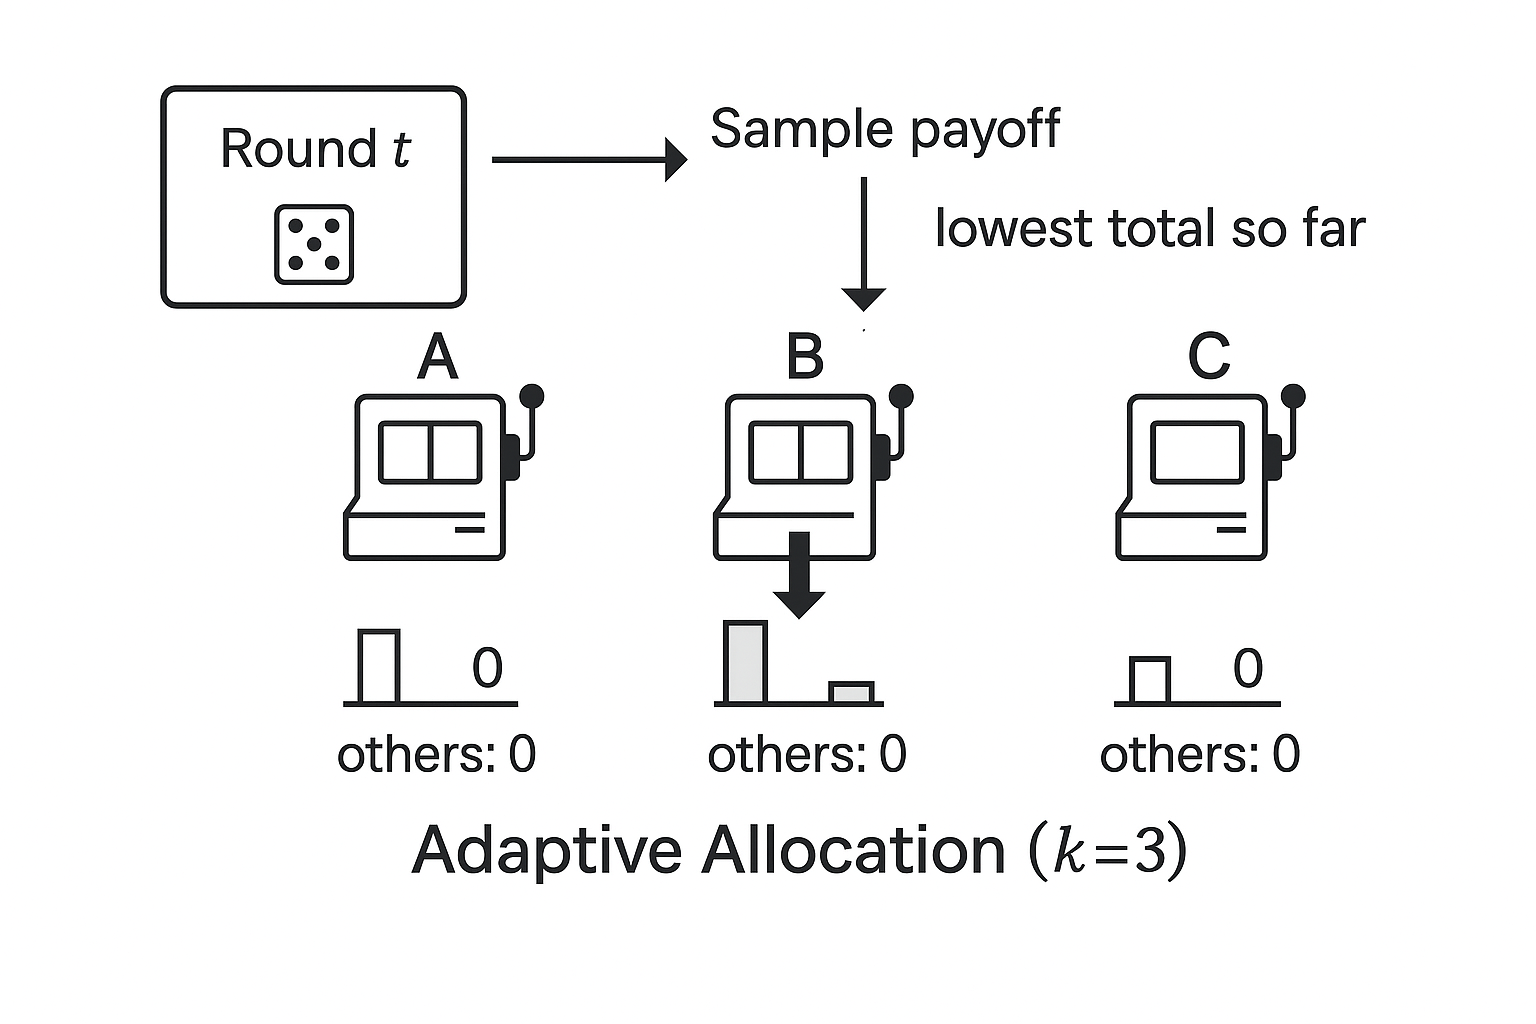
\includegraphics[width=0.3\linewidth]{332Project2//figures/Image_A.png}
        \caption{Image of A}
        \label{fig:placeholder}
    \end{figure}
\end{frame}


\begin{frame}{A - Results(Regret)}
\textbf{Results}\\
Here is a graph showing the change in regret. \\
We conclude that these results are consistent with the intuition. The result show that in FTL regret increase linear in rounds, while the other's regret are almost zero.
\begin{center}
    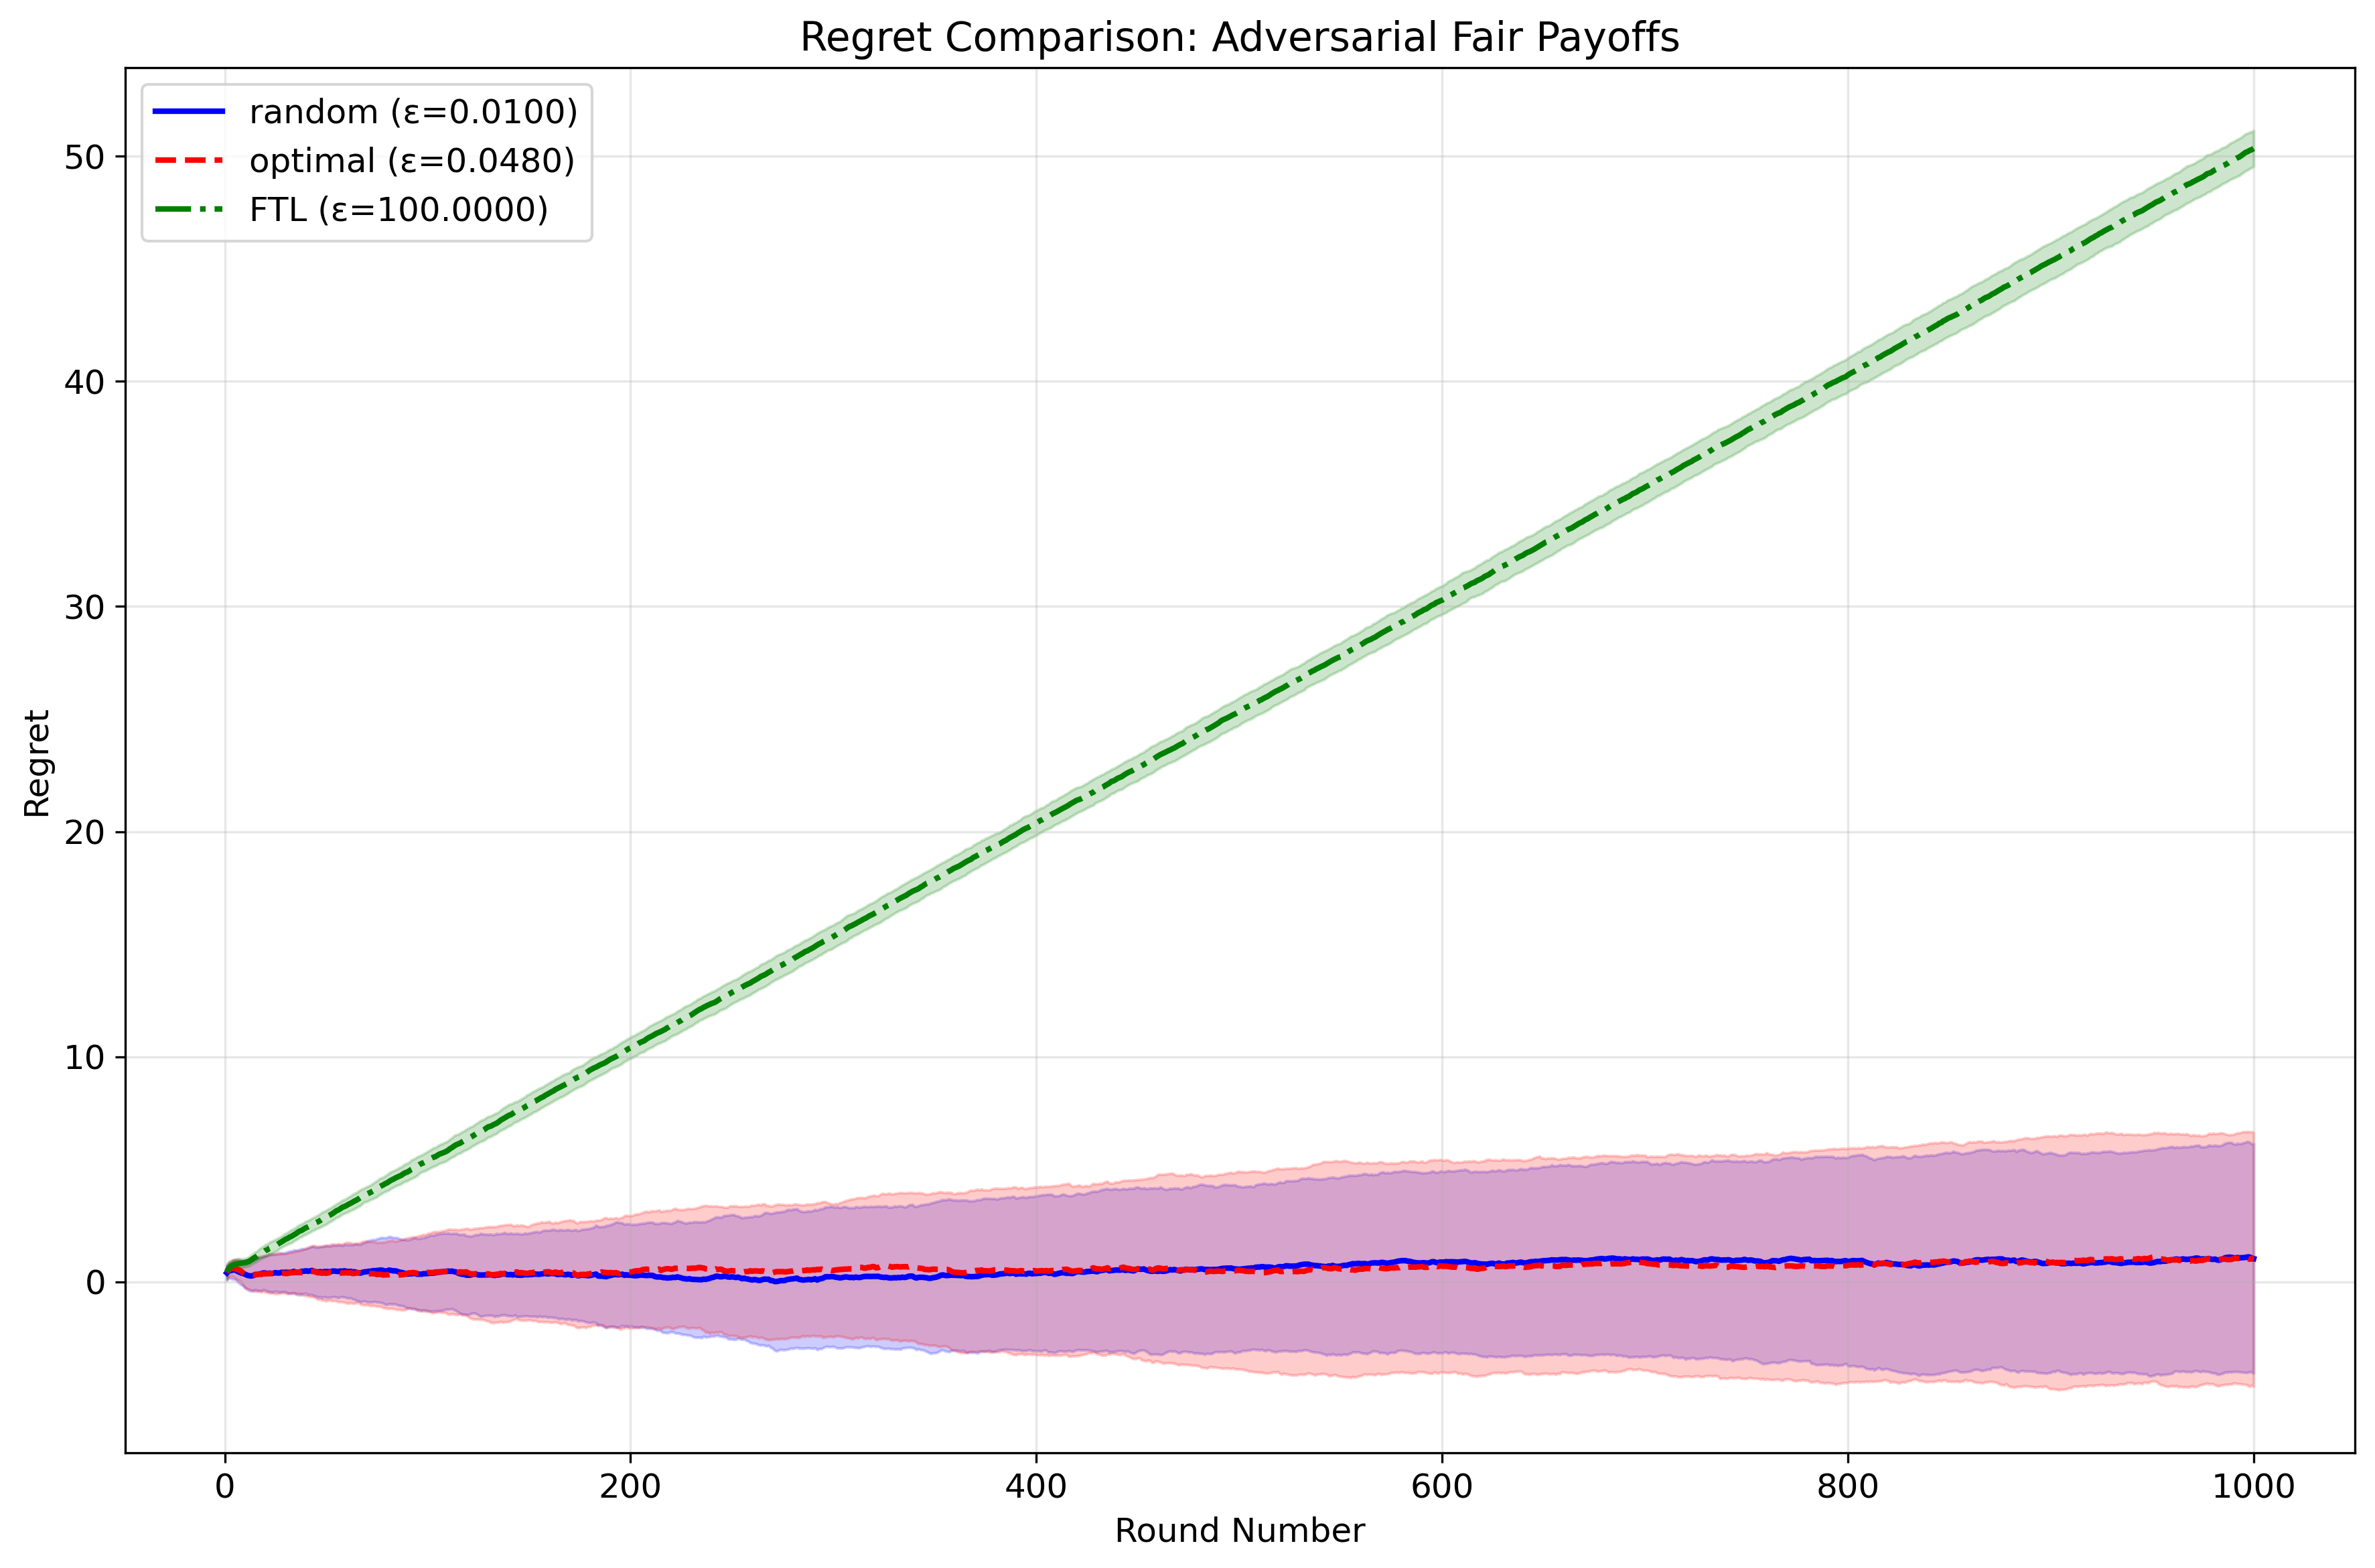
\includegraphics[width=0.7\textwidth]{332Project2/figures/adversarial_regret_comparison.png}
\end{center}
\end{frame}


\begin{frame}{A - Additional Analysis on Results}
\textbf{FTL}\\
Strictly speaking, FTL in AFP can be described as follow; 
each round, FTL regret what he did, then he learn that optimal past total payoff, he choose the action whose total payoff in past is the most, which points O at next round, so that's why his regret increases linearly in rounds.
Excemption: it is possible that action with smallest total payoff be with smallest total payoff even if add points. In this exemption, FTL works.
\textbf{random}\\

\textbf{optimal}\\

\end{frame}

\begin{frame}{A - Results(Payoffs)}



\end{frame}

\begin{frame}{A - Results(Regret Bound)}
    According to the setting, regret bound of optimal learning rate is
    \[
    Regret_t \leq 2 * 1 * \sqrt{1000log3} \approx 110
    \]
    we can easily see that regret is binded by this bound.
\end{frame}

\subsection{B : BP}

\begin{frame}{B - Setting:}
    Next, BP.\\
    Fix a probability for each action $p_{1},...,p_{k}$ with each $p_{k}$ in [0,1/2].\\
    In each round i,
    \begin{itemize}
        \item draw the payoff of each action j as $v^{i}_{j} \sim B(p_{j})$ (i.e, from the Bernoulli distribution with probability $p_j$ of being 1 and probability $1-p_{j}$ of being 0).
    \end{itemize}
    \vspace{1em}
    Here's our parameters;
    \begin{itemize}
        \item k = 3
        \item n = 1000
    \end{itemize}
\end{frame}

\begin{frame}{B - Game structure and Intuition}
    Here's game structure and out intuition is that 
    \begin{itemize}
        \item since there are fixed probability, FTL will find the best machine with highest probability earliest
        \item while optimal will slowly approaching toward the best machine and random will work poorly.
    \end{itemize}
    \begin{figure}
        \centering
        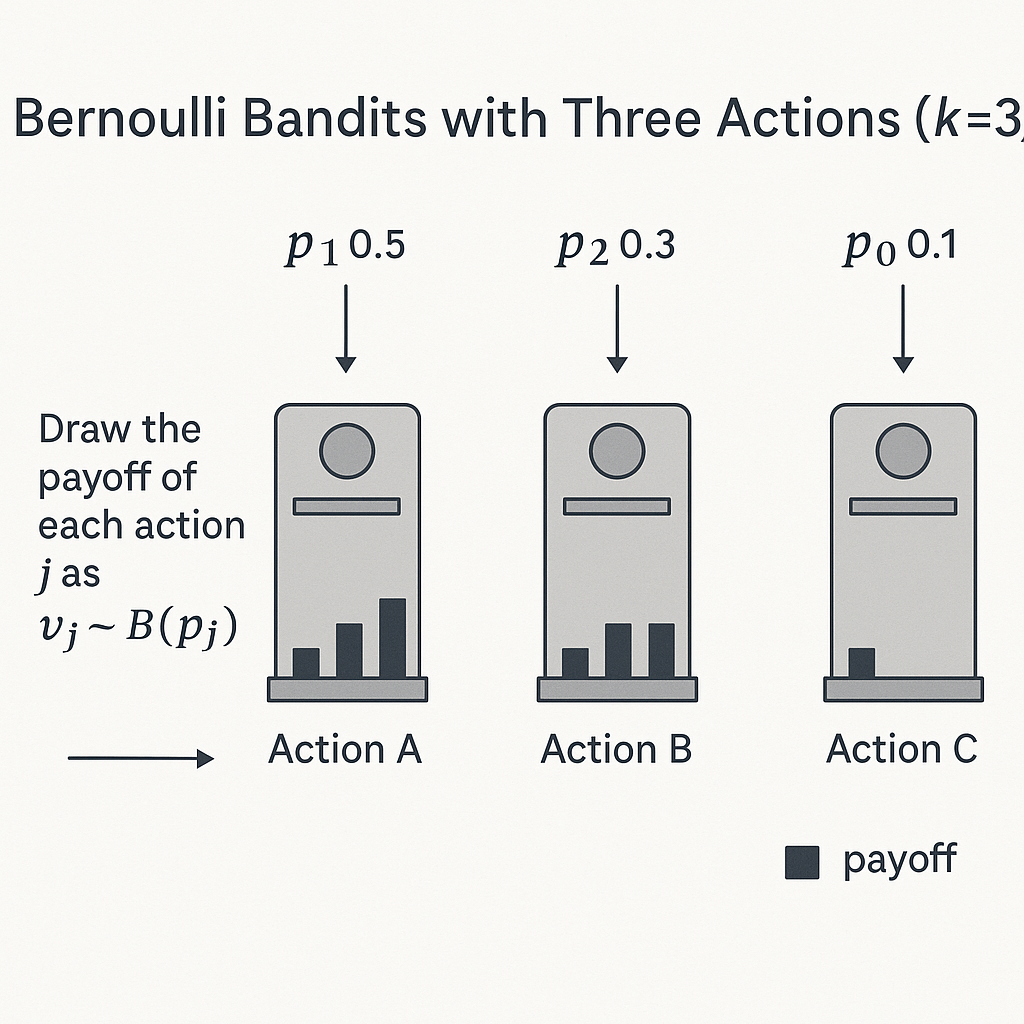
\includegraphics[width=0.4\linewidth]{332Project2//figures/Image_B.png}
        \caption{Image of B}
        \label{fig:placeholder}
    \end{figure}
\end{frame}

\begin{frame}{B - Results(Regret)}
\textbf{Results}\\
Here is a graph showing the change in regret. \\
We conclude that these results are consistent with the intuition. \\
\begin{center}
    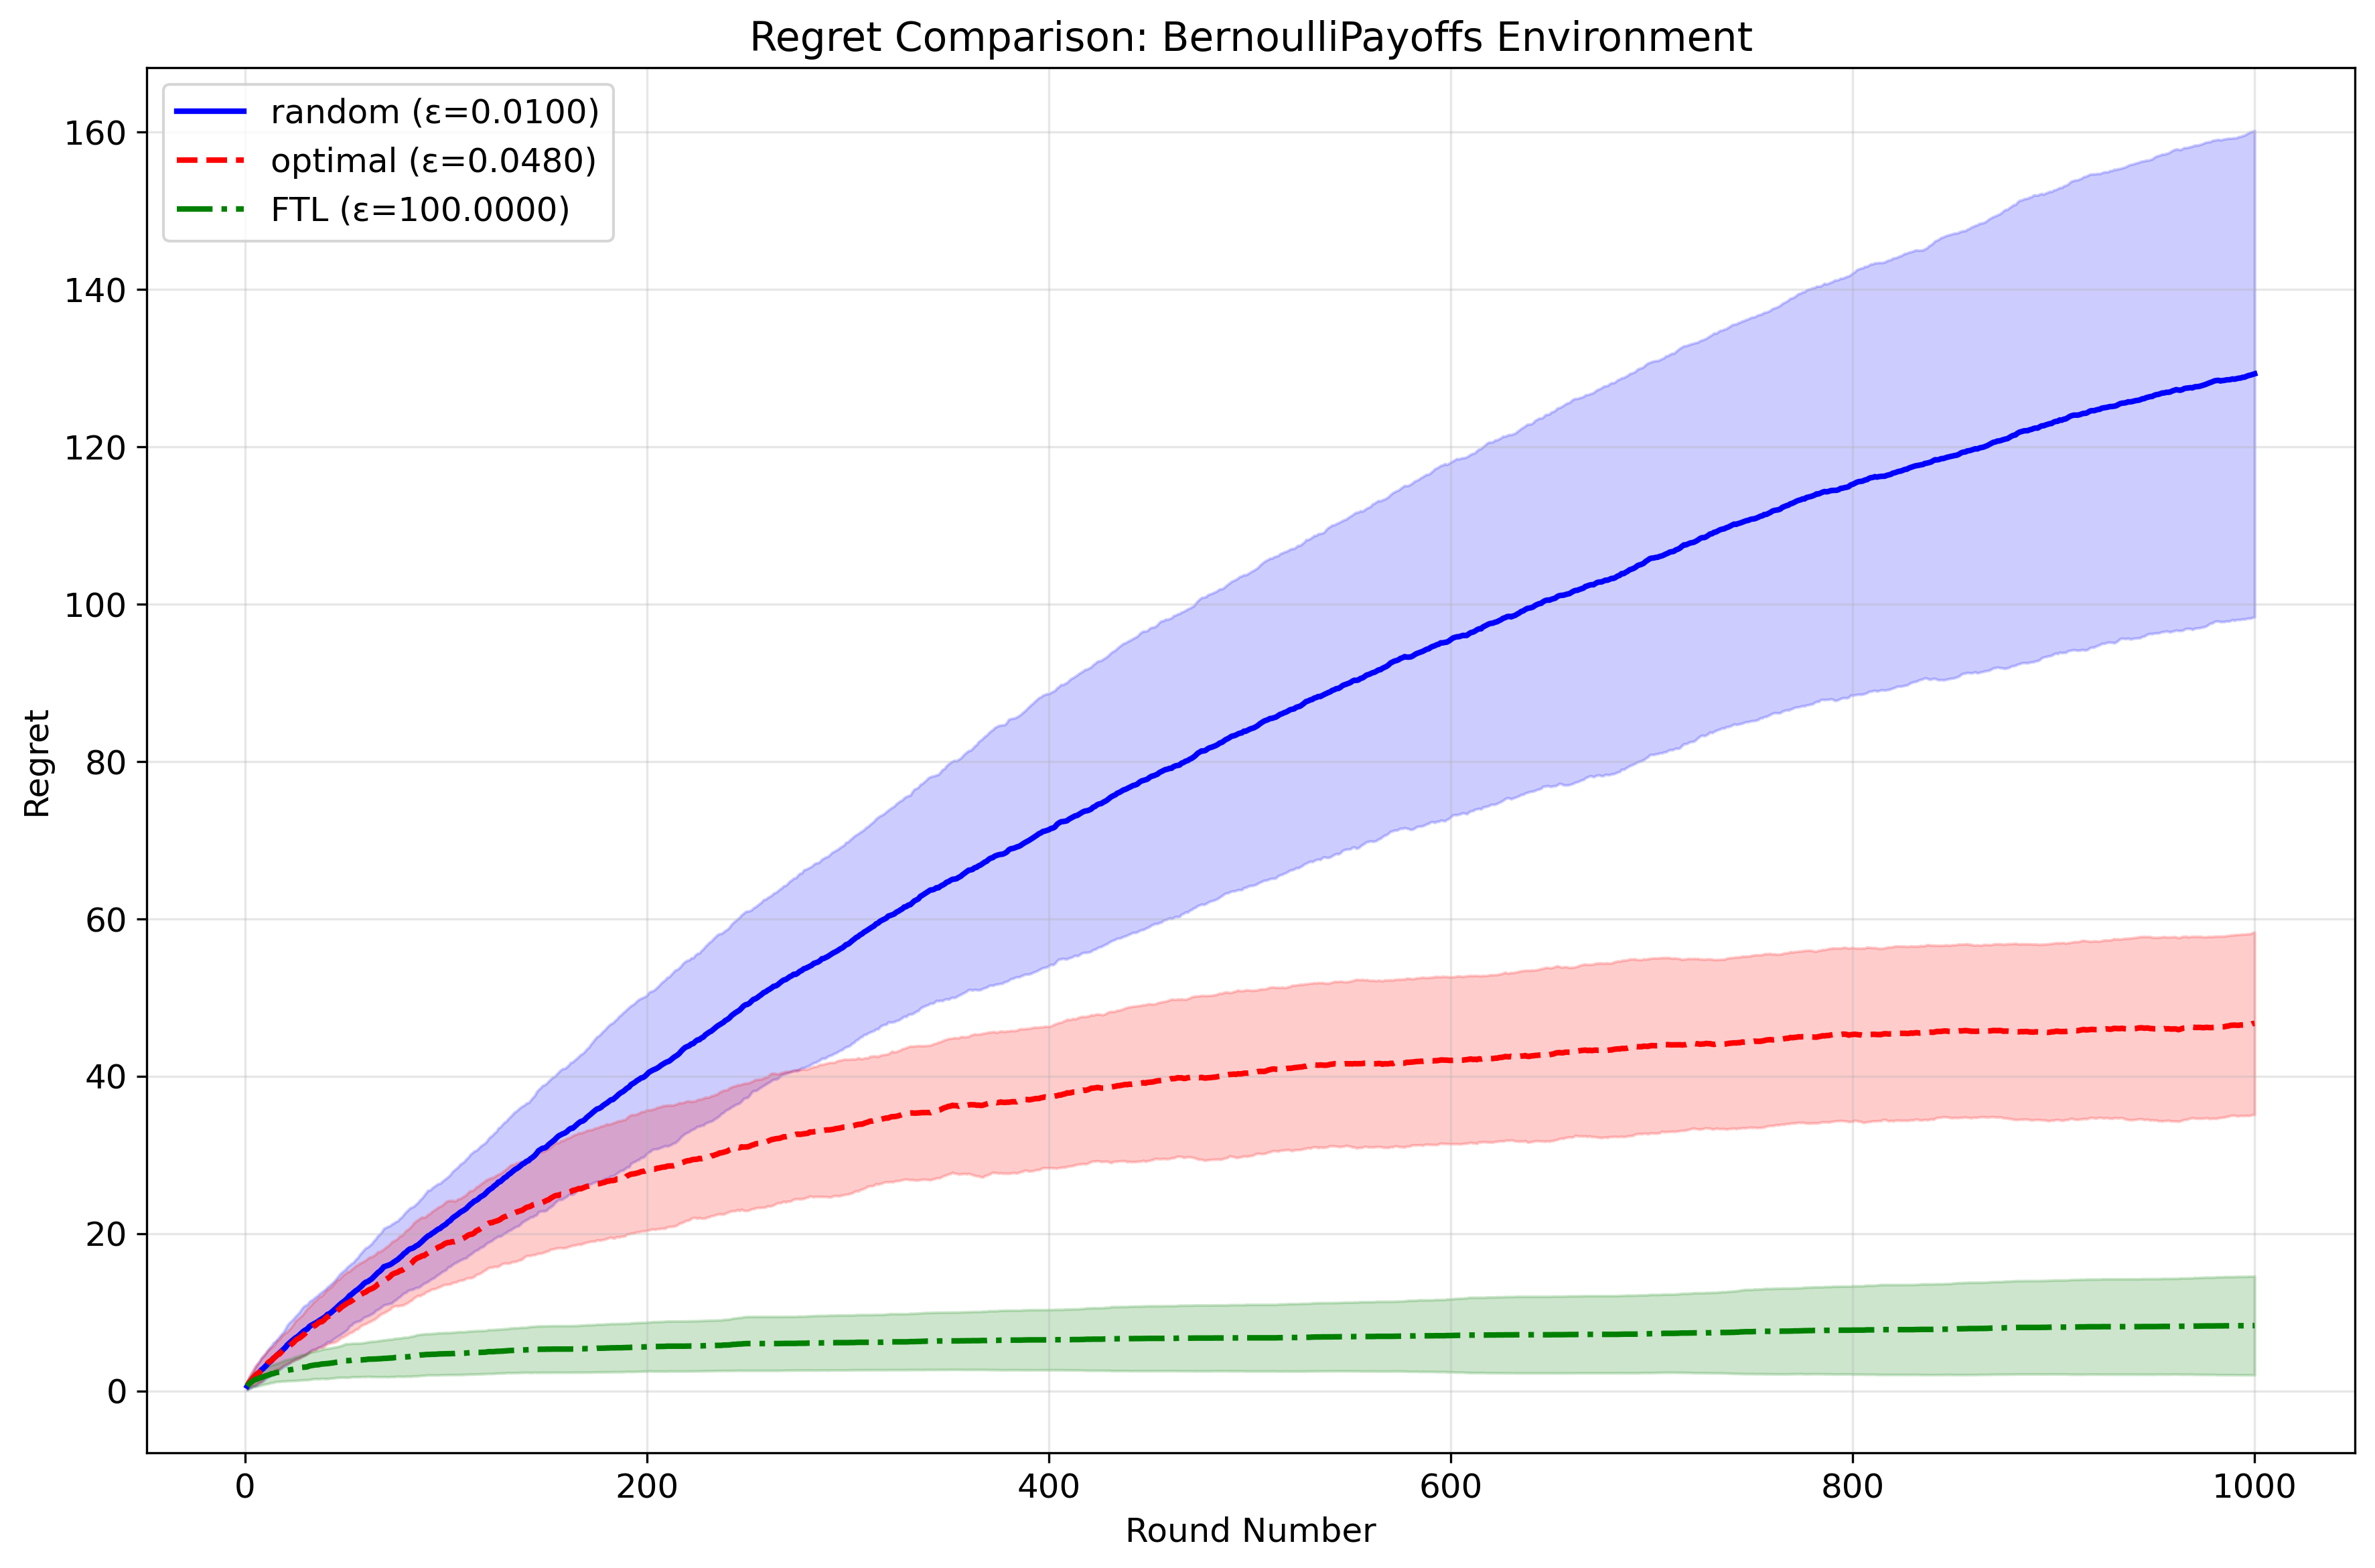
\includegraphics[width=0.5\textwidth]{332Project2/figures/bernoulli_regret_comparison.png}
\end{center}
\end{frame}

\begin{frame}{B - Additional Results}
\textbf{Results}\\
To support our initial intuitive, we get another results about ranking
possibility of local optima.because 95 CI so huge.
\begin{center}
    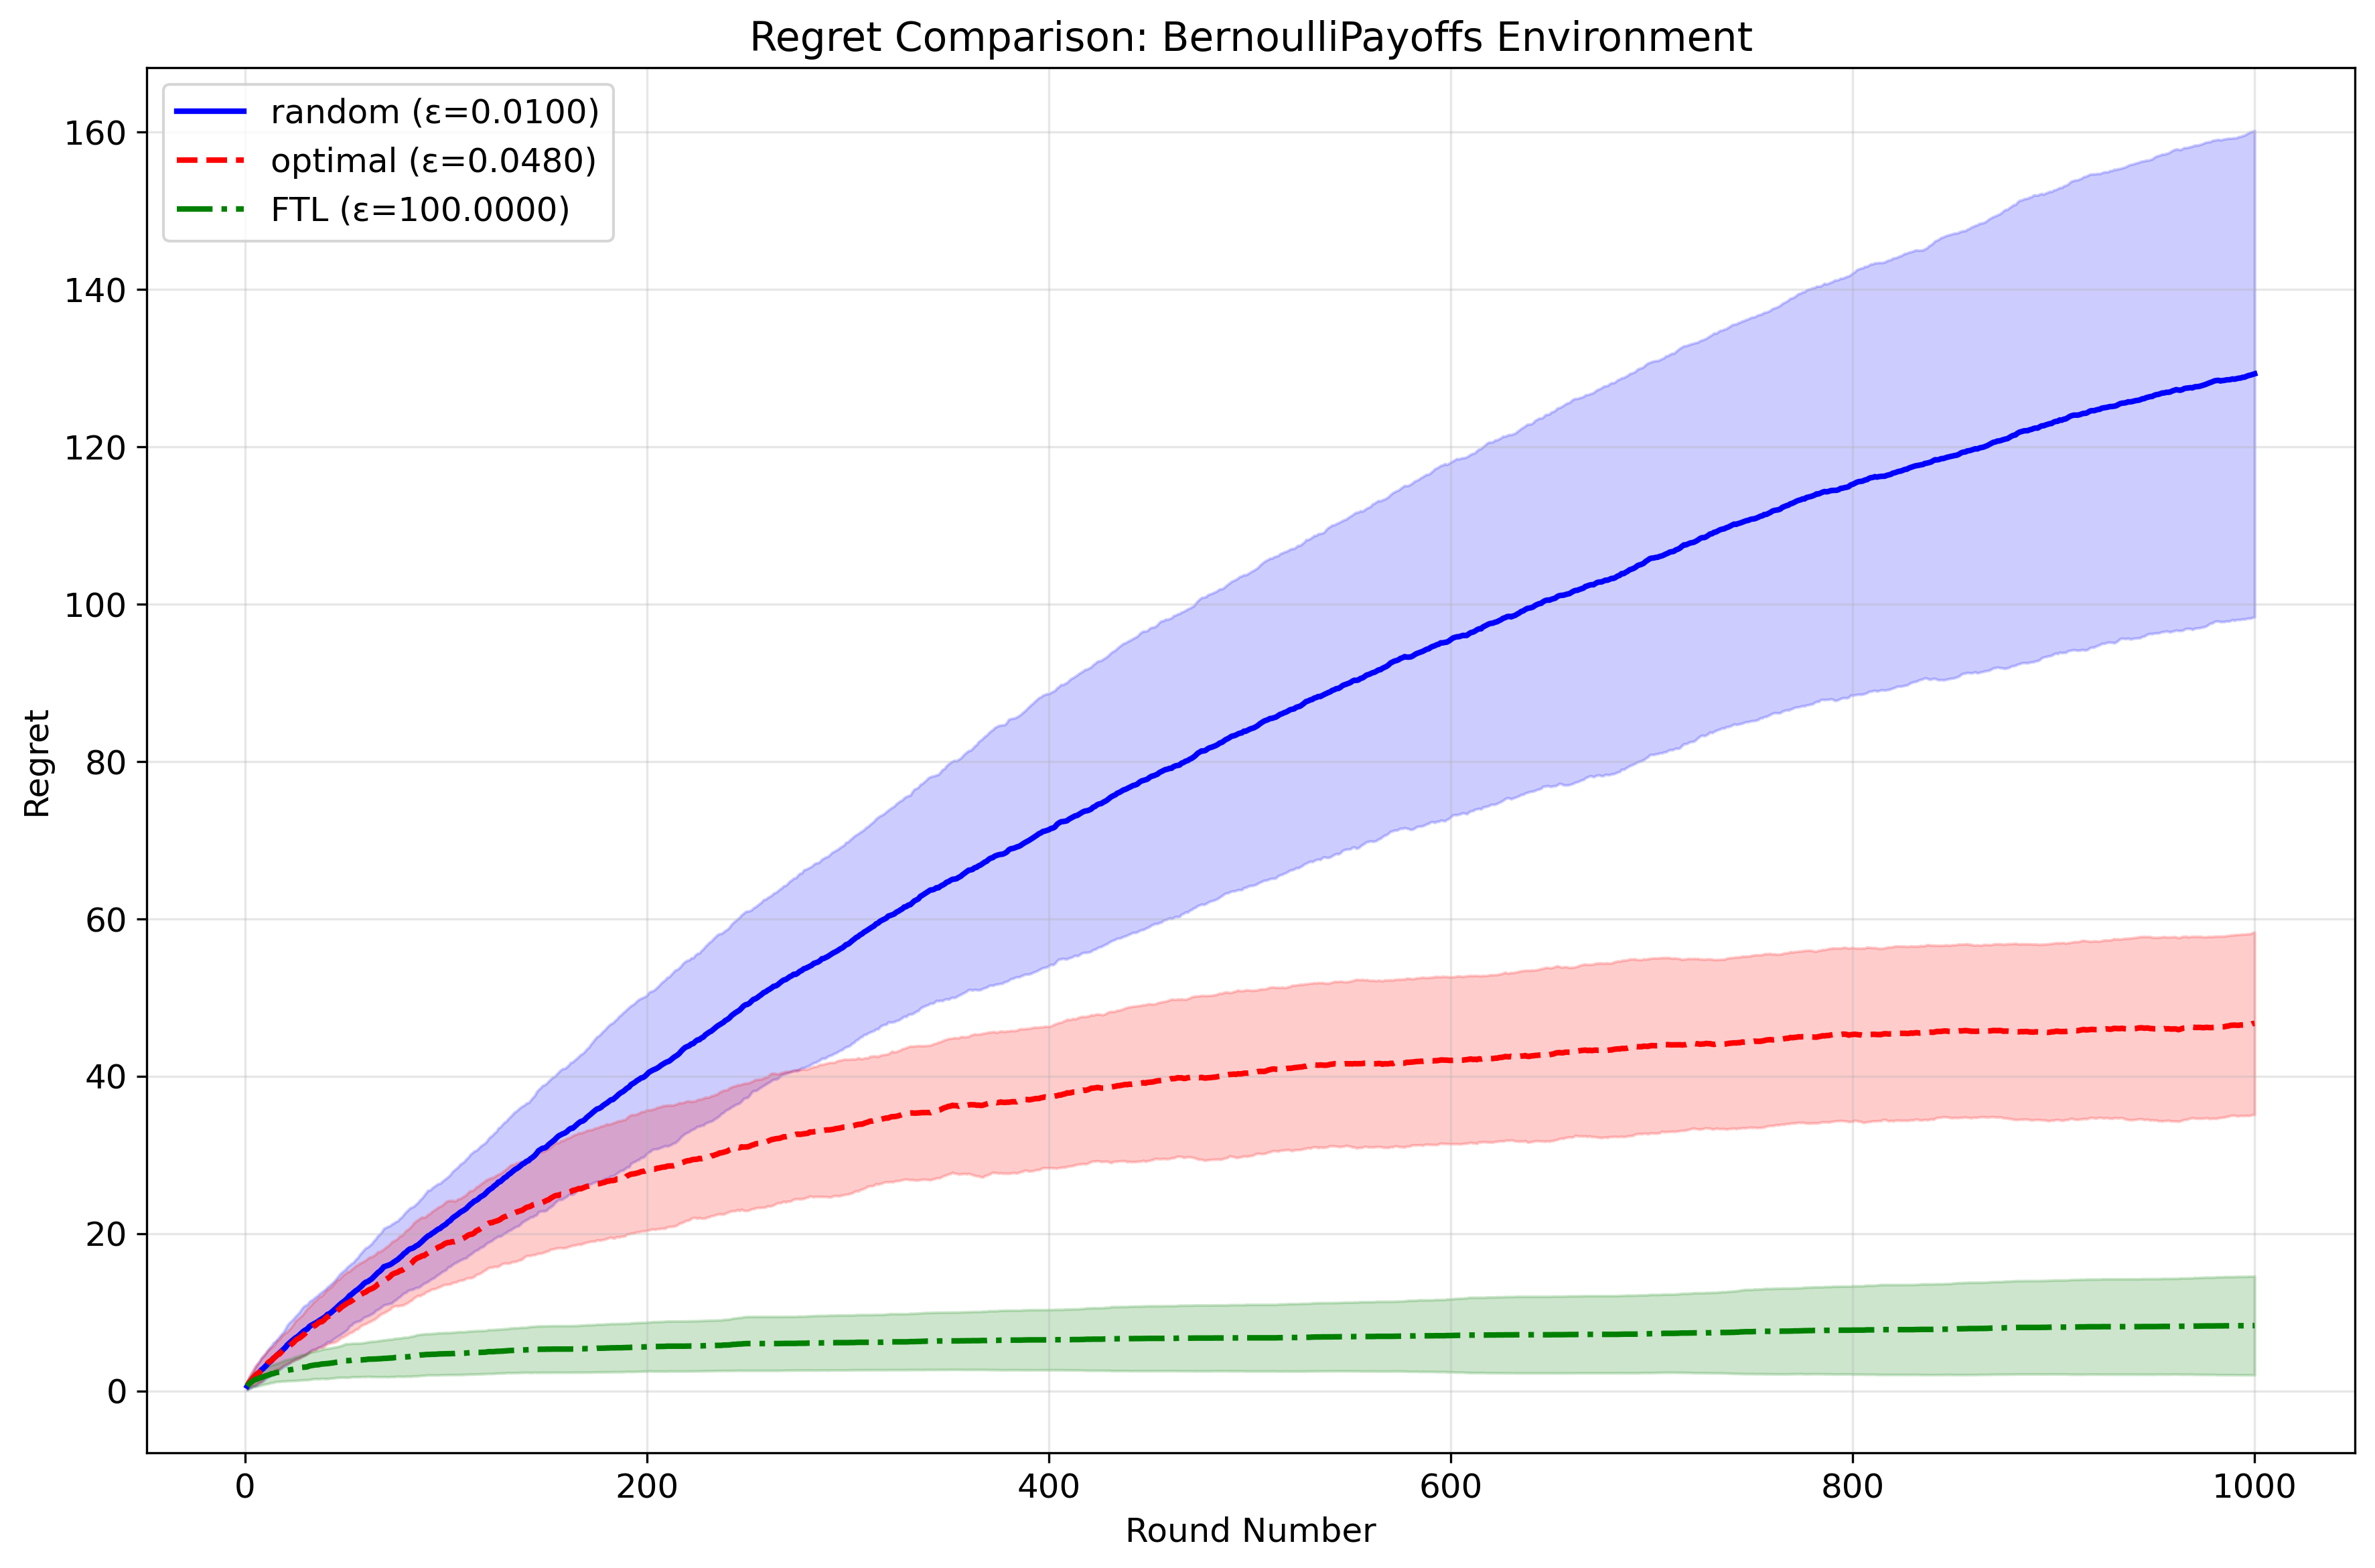
\includegraphics[width=0.5\textwidth]{332Project2/figures/bernoulli_regret_comparison.png}
\end{center}
\end{frame}

\begin{frame}{B - Additional Results}
what if k increases, it must leads FTL to local optima.  NO\\
Because FTL has mechanism that choose 
\[
\frac{\text{total payoff}_j}{\text{rounds}_j} \approx p_j \quad n \rightarrow\infty
\]
which means FTL finds machines with the higest possibility.
\begin{center}
    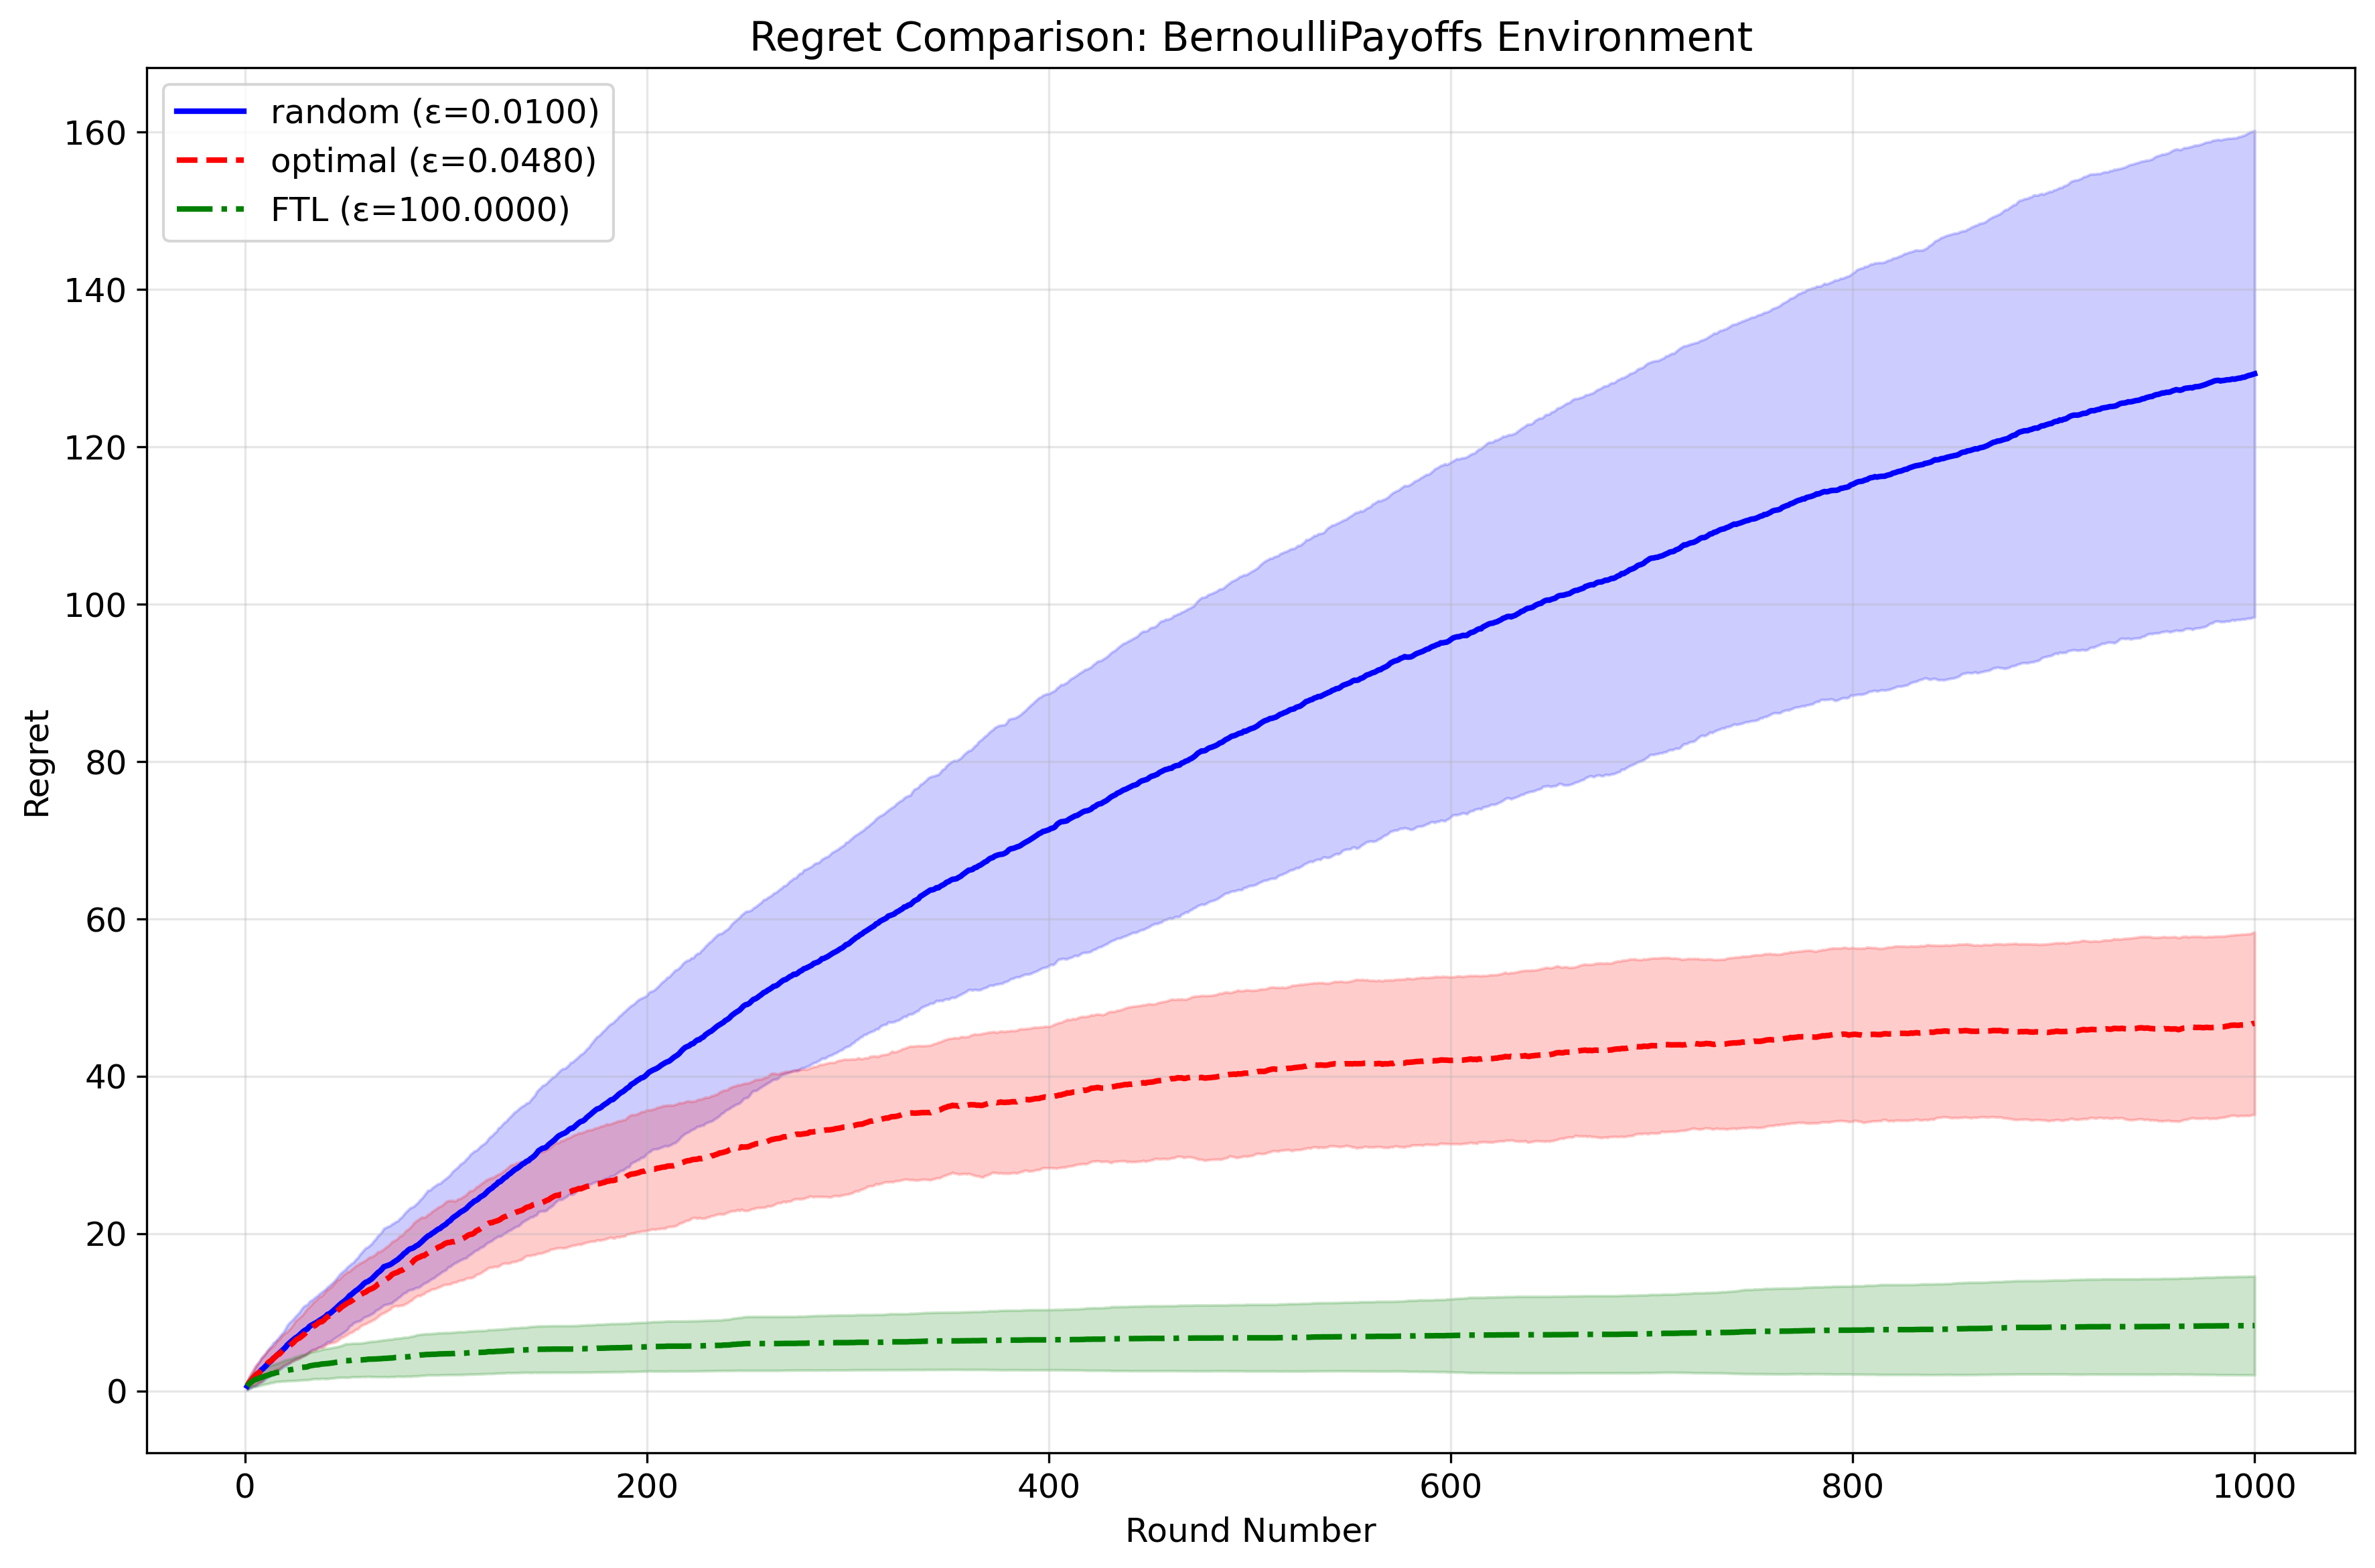
\includegraphics[width=0.5\textwidth]{332Project2/figures/bernoulli_regret_comparison.png}
\end{center}
\end{frame}

\begin{frame}{B - Results(Payoffs)}
\textbf{Results}\\
Calculating total payoffs in this setting. it is consistent with result
\begin{center}
    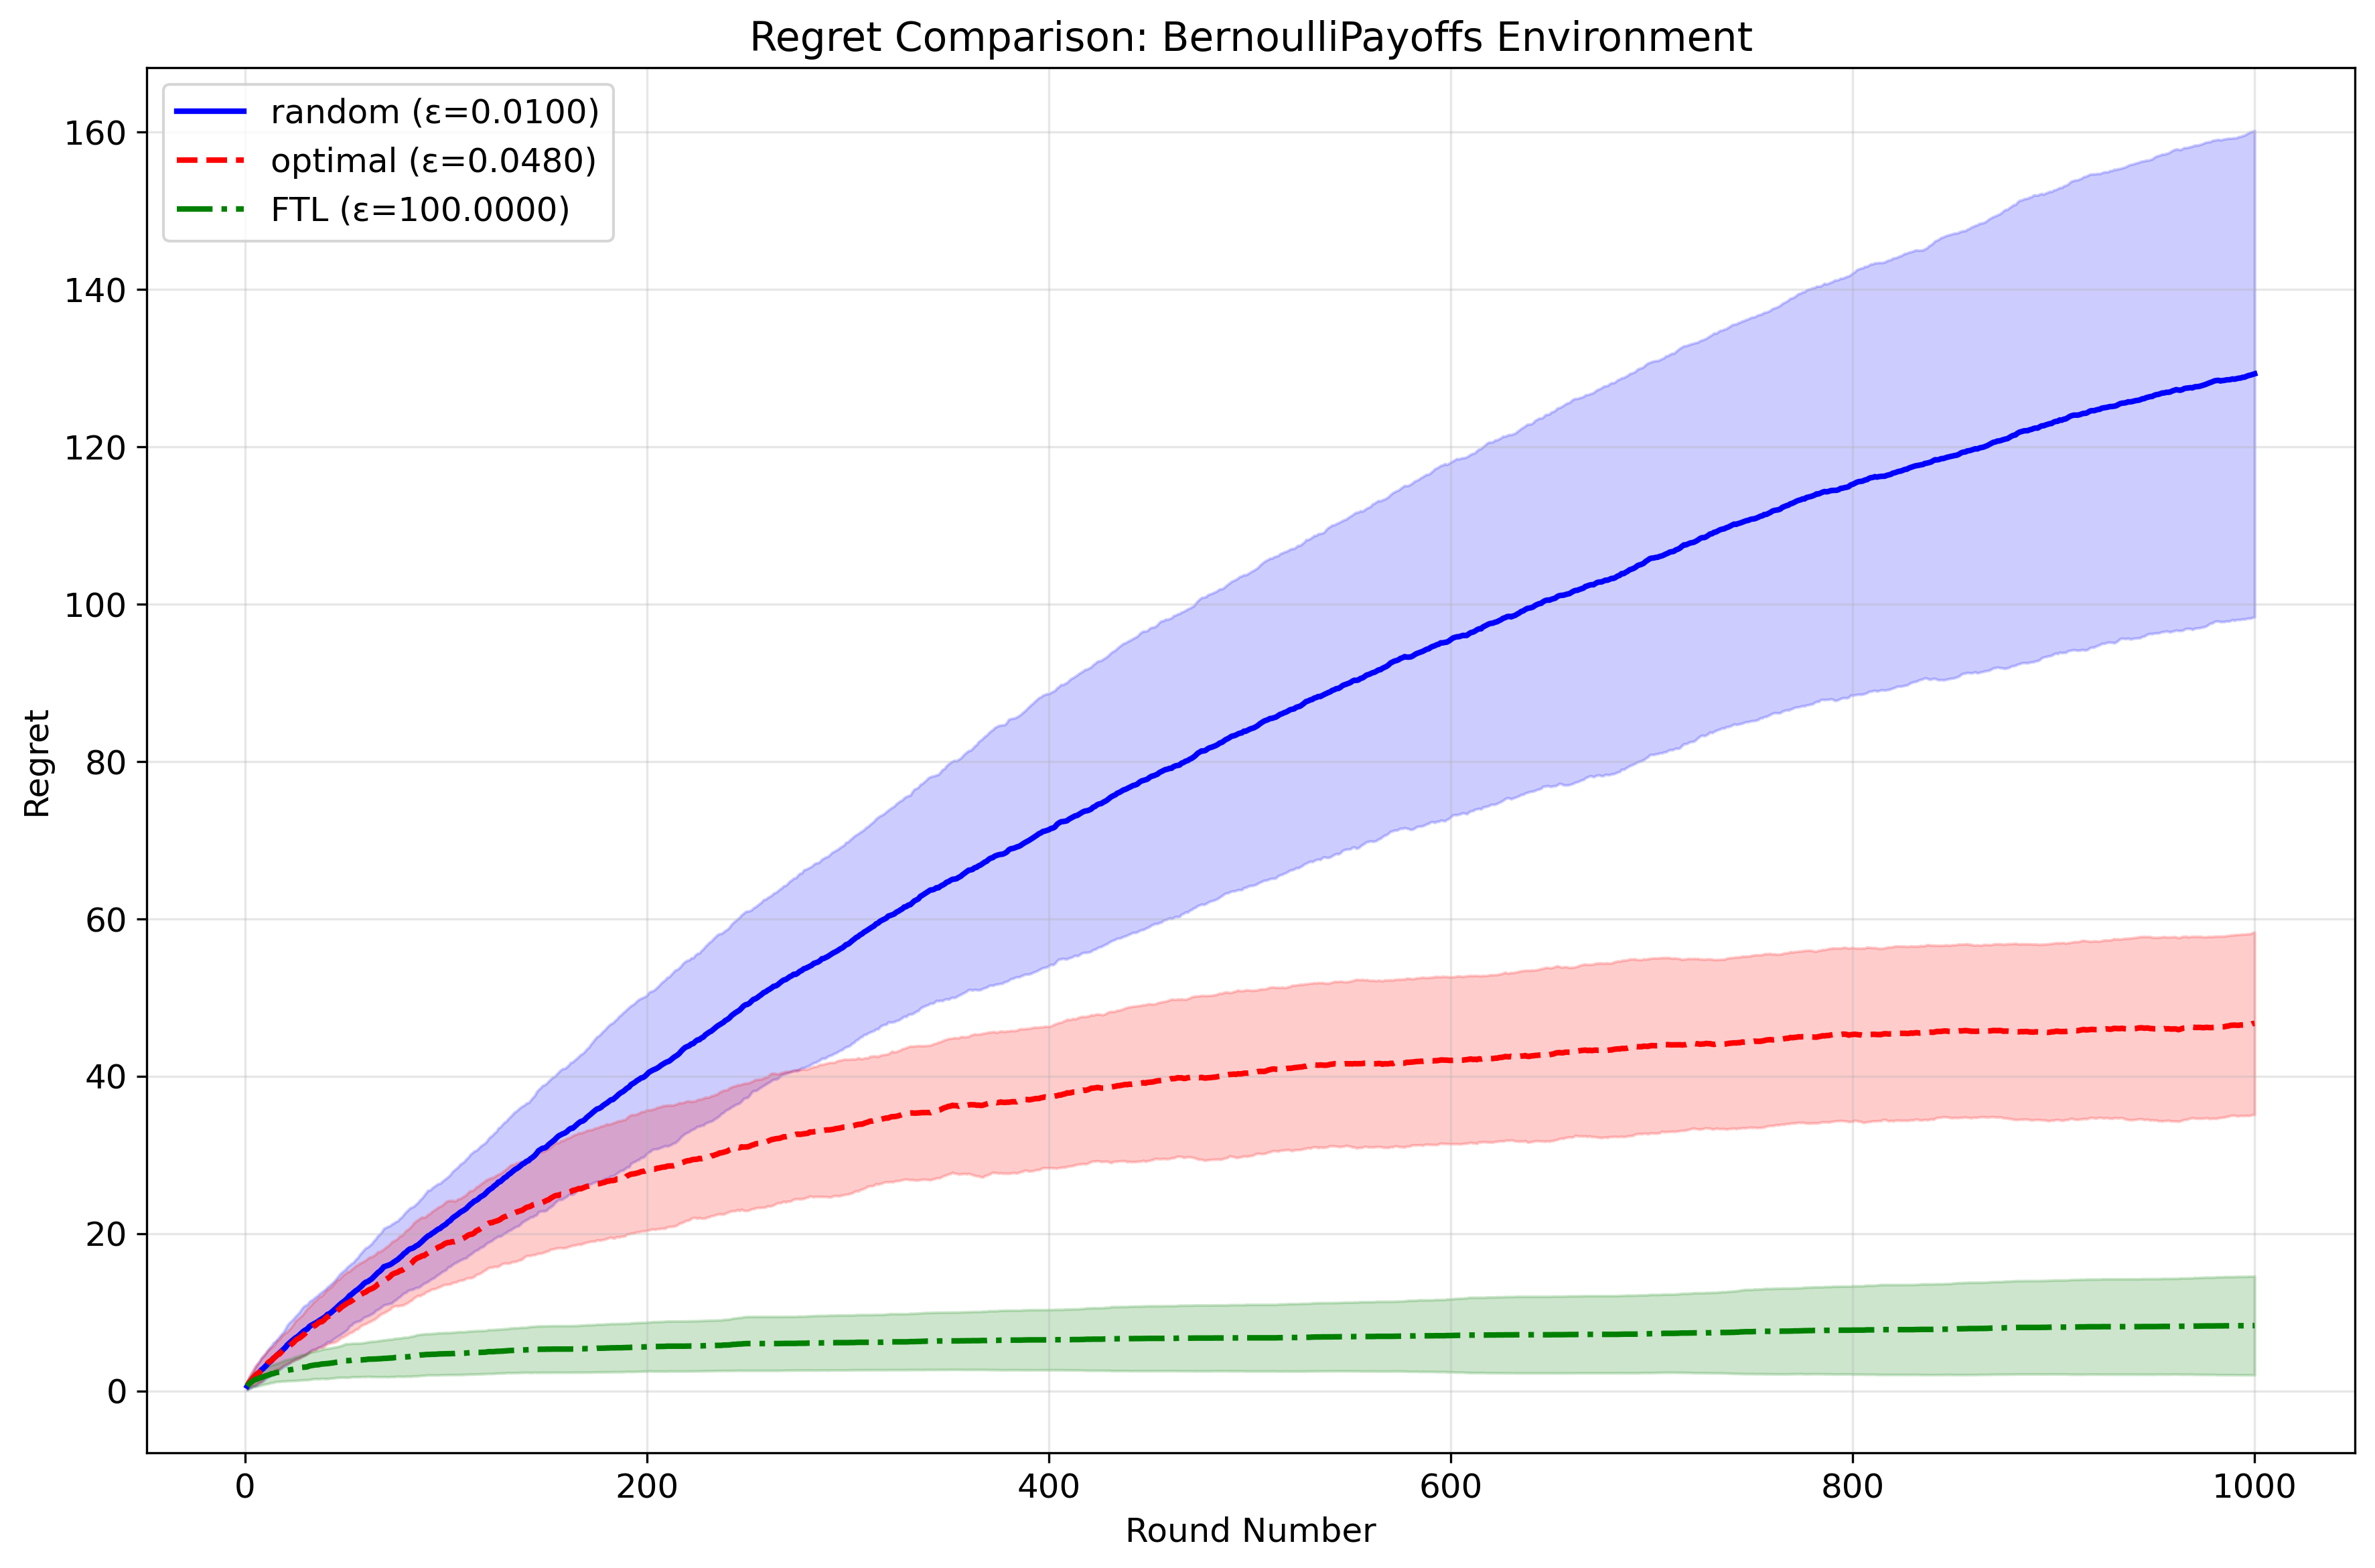
\includegraphics[width=0.5\textwidth]{332Project2/figures/bernoulli_regret_comparison.png}
\end{center}
\end{frame}

\begin{frame}{B - Results(Regret bound)}
\textbf{Results}\\
    According to the setting, regret bound of optimal learning rate is
    \[
    Regret_t \leq 2 * 1 * \sqrt{1000log3} \approx 110
    \]
\begin{center}
    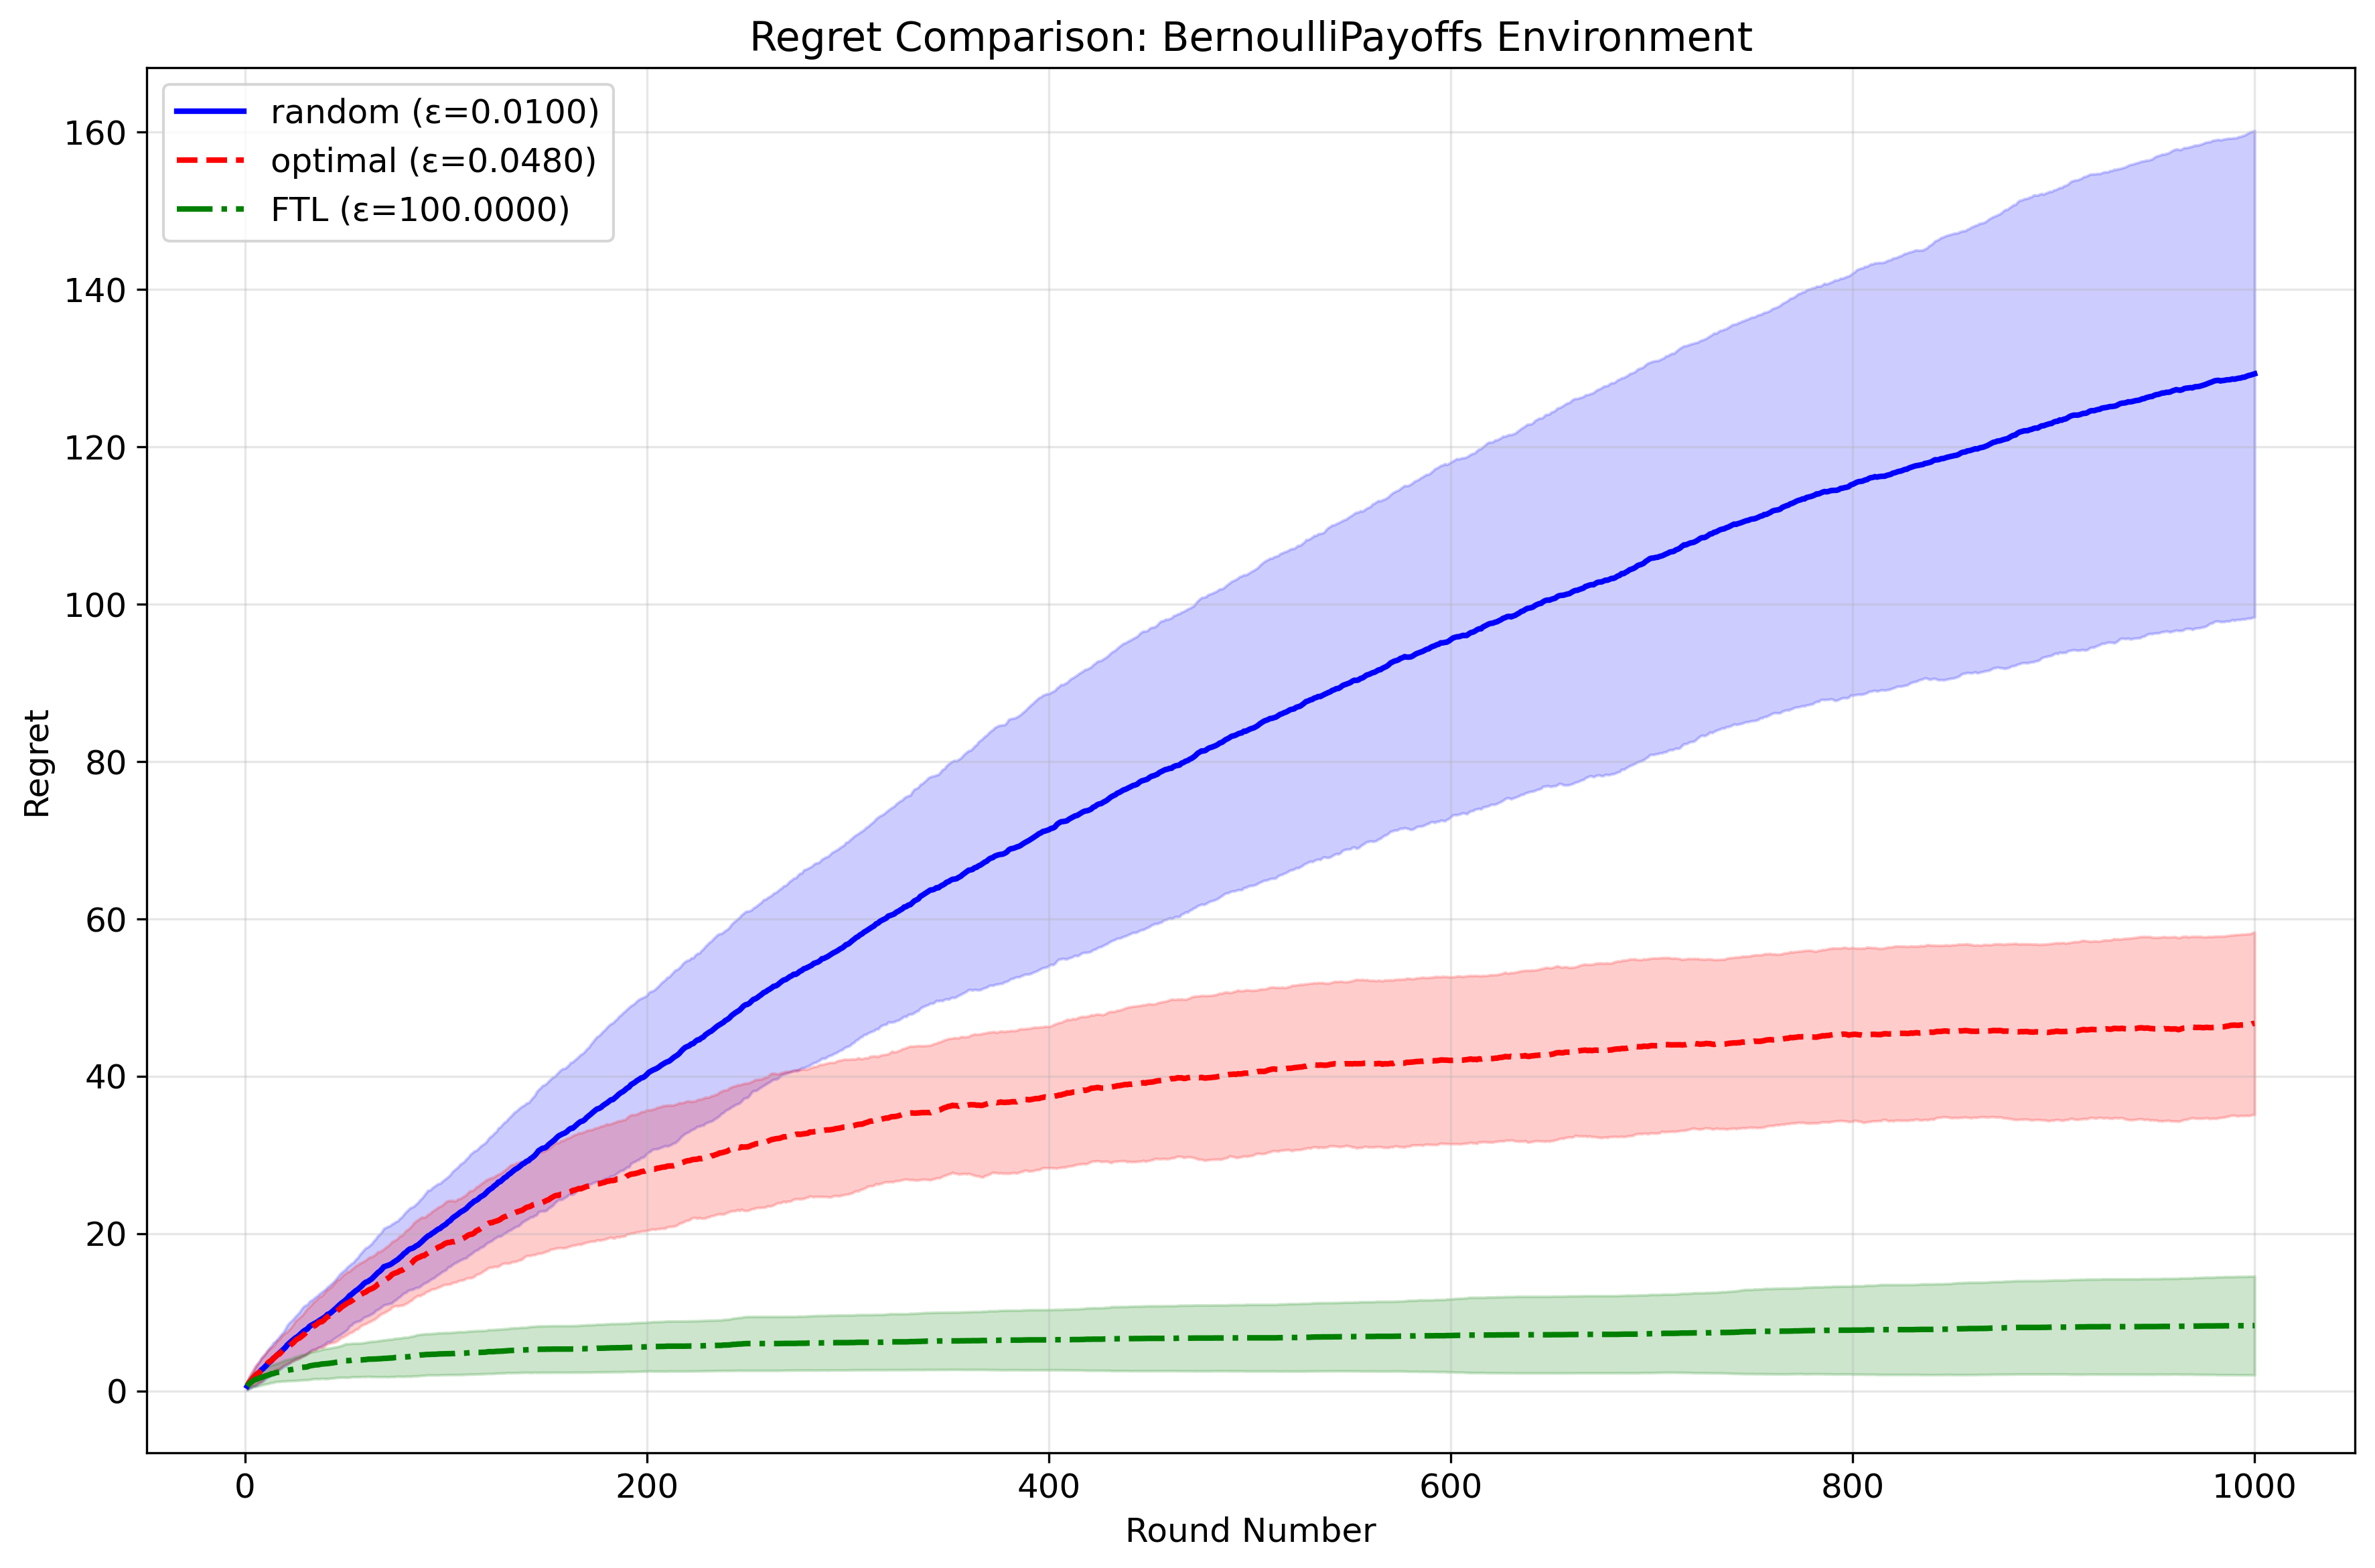
\includegraphics[width=0.5\textwidth]{332Project2/figures/bernoulli_regret_comparison.png}
\end{center}
\end{frame}


\section{Part2}


\begin{frame}{Part2 - Outline}
In Part 2, we consider two things;
\begin{enumerate}
    \item Data in the Wild
    \begin{itemize}
        \item EW algorithm applied to Pachinko Payoffs (hereinafter abbreviated as "PP")
        \item we used data from Pachinko
    \end{itemize}
    \item Adversarial Generative Model
    \begin{itemize}
        \item Research Payoffs (hereinafter abbreviated as "RP")
        \item we modeled our Researcher's decision to review the previous researches in online learning framework.
    \end{itemize}
\end{enumerate}
\end{frame}

\subsection{C : PP}

\begin{frame}{Part2-C - Summary}
\textbf{Methods}\\
In part C, Using unique data from Japanese Pachinko, and formulate the problem of store selection.  

\vspace{1em}
\textbf{Results}\\
FTL's regret converges to 0, while the others performs poorly.

\vspace{1em}
\textbf{Takeaways}\\
From limited data, we show the optimality of common strategies.
\end{frame}

\begin{frame}{C - Description of Pachinko}
    In this part, we describe Japanese Pachinko.\\
    {\small
    \textbf{general description}:\\
    Pachinko is \textbf{a Japanese gambling-like game} that uses small steel balls, which can be exchanged indirectly for money. A pachinko machine can be modeled as a stochastic system that draws payoffs from fixed probabilities, often involving state transitions\\
    \vspace{1em}
    While we could not obtain empirical data from actual machine logs on the scale of thousands of plays, we discovered \textbf{another interesting dataset} that captures related dynamics.}
    \begin{figure}
        \centering
        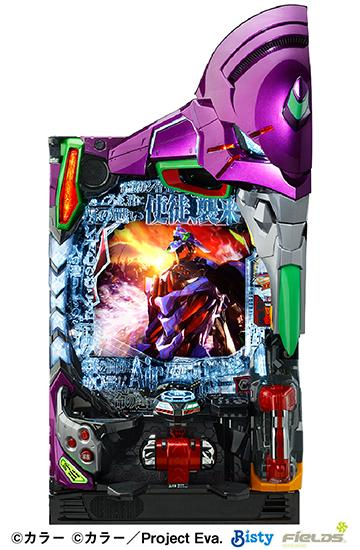
\includegraphics[width=0.15\linewidth]{332Project2//figures/machine_evangelion.jpg}
        \caption{Machine Example}
        \label{fig:placeholder}
    \end{figure}
\end{frame}

\begin{frame}{C - Description of Data}
Here is Description of Data.\\
\textbf{Data}:\\
Pachinko stores publicly report daily ball counts (in/out), so we can calculate daily average ROI (Return Of Investment) from this data.\\
\vspace{1em}
Two characteristics align with the modeling choice:
\begin{itemize}
  \item \textbf{Aggregation:} Store-level ROI is a coarse proxy for machine-level profitability, but it is observable and comparable across stores day by day.
  \item \textbf{Nonstationarity:} Stores strategically change settings to attract customers or to gain profit, so payoffs can be nonstationary.
\end{itemize}
we choose 5 stores in major cities in Tokyo.
\end{frame}

\begin{frame}{C : Time series of daily ROI}
Below is the time series of daily ROI in each store, showing the characteeristic of nonstationarity.
    
\end{frame}

\begin{frame}{C - Appendix}
    \textbf{Excuse}\\
    This formulation of problem is not far from the real-world strategy. We use data which is trusted among this community in Japan. In addtion, Practitioners often aggregate and forecast store-level returns, sometimes coordinating group play.\\
    This motivates treating each store as an “arm" and applying Exponential Weights Algorithm to store choices rather than to individual machines. 
\end{frame}

\begin{frame}{C - Data}
    Here's how we use data.\\
    \begin{itemize}
        \item \textbf{ROI Data define Payoffs.}\\
    Let stores $s\in\{1,\dots,S\}$ (e.g.\ $S=5$) and days $i=1,\dots,I$.\\
    From data, for each $(s,i)$ observe balls-in/out and total balls:
    \[
    B^{\text{in}}_{s,i},\quad B^{\text{out}}_{s,i},\quad T_{s,i}>0.
    \]
    Define raw ROI and a per-day normalized payoff in $[0,1]$:
    \[
    r_{s,i}\;=\;\frac{B^{\text{out}}_{s,i}-B^{\text{in}}_{s,i}}{ T_{s,i}},\qquad
    v_{s,i}\;=\;\frac{r_{s,i}-\underline r_i}{\overline r_i-\underline r_i+\varepsilon}\in[0,1],
    \]
    where $\underline r_t=\min_{j} r_{j,i}$, $\overline r_i=\max_{j} r_{j,i}$, and $\varepsilon>0$ is small.
    \end{itemize}
\end{frame}

\begin{frame}{C - Setting}
In each day i, Player
\begin{enumerate}
  \item Choose a store $s_i$ 
  \item from data Extract ROI as $v_{s,i}$
\end{enumerate}
\vspace{1em}
So, it's a simple setting of player choosing stores among 5 stores under full-information.

\end{frame}

\begin{frame}{C - Game Structure and Intuition}
Here's our Intuition;
\begin{itemize}
    \item It seems like it is best to go to the store with highest ROI yesterday like FTL (most Japnese do)
    \item However, there's possibility that stores strategically change minor setting of machines to lower ROI, so that they gain profit. 
\end{itemize}
\begin{figure}
    \centering
    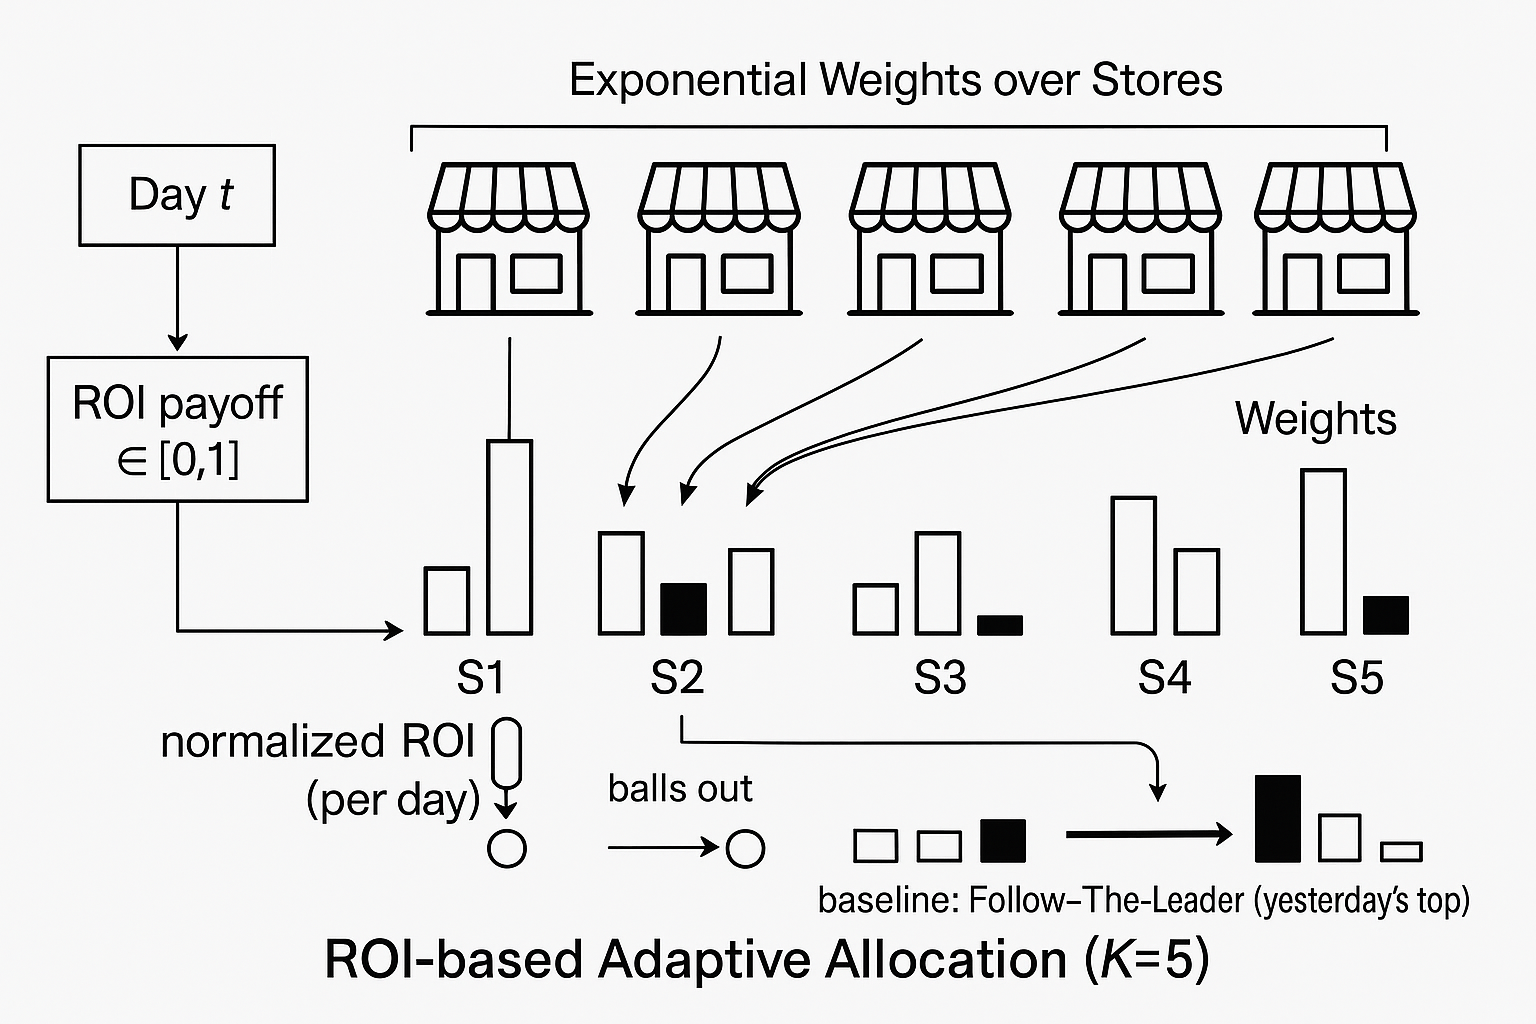
\includegraphics[width=0.4\linewidth]{332Project2//figures/Image_C.png}
    \caption{Image of C}
    \label{fig:placeholder}
\end{figure}

\end{frame}

\begin{frame}{C - Results(Regret)}

    
\end{frame}


\begin{frame}{C - Results(Payoffs)}

    
\end{frame}

\begin{frame}{C - Results(Regret bound)}

    
\end{frame}



\subsection{D : RP}

\begin{frame}{Part2-D - Summary}

\textbf{Methods}\\
We formulate a (randomized) data generating model for where neither FTL nor uniform guessing have vanishing regret by introducing Cluster structure and regime change into normal paper search model, which is consistent with a real world.

\vspace{1em}
\textbf{Results}\\



\vspace{1em}
\textbf{Takeaways}\\


\end{frame}

\begin{frame}{D - Motivation}
I have two motivations(technical and private) to formulate a new data generating model.
    \begin{itemize}
        \item \textbf{Technical} : N-dimensional maximization
        \begin{itemize}
            \item In simple setting, "arm" is one-dimensional with one-dimensional payoff. Motivated by ps3 problem 1, we extend it to N-dimensional maximization(in practice N=20).
        \end{itemize}
        \item \textbf{Private} : My experience as Research Assistant
        \begin{itemize}
            \item In research, we have to review lots of previous reseach not knowing the whole picture of fields. We have to distribute effort to each papers, which sometimes is trash for your research, sometimes treasure for your research.
        \end{itemize}
    \end{itemize}
\end{frame}


\begin{frame}{D - Techniques}
    In academic world, there are two often-said characteristics
    \begin{itemize}
        \item \textbf{High-quality papers are mass-produced by a cluster of researchers}
        \begin{itemize}
            \item we can formulate this by introducing correlation of paper's value in a cluster
            \item which disturbe uniform guessing to be optimal and to converge to the no-regret condition
        \end{itemize}
        \item \textbf{Frequent innovations (regime changes) in research methods}
        \begin{itemize}
            \item we can formulate this by introducing possibility of regime change 
            \item which disturbe FTL to be optimal and to converge to the no-regret condition
        \end{itemize}
    \end{itemize}
    Our technique leverages these well-known properties to formulate online learning in a way that suits the conditions of our problem.
\end{frame}

\begin{frame}{D - Setting}
In each round $i$:
\begin{enumerate}
    \item Draw a latent \textbf{regime state} $z_i \in \{1, \dots, m\}$,
          which represents the ``active cluster'' of useful literature.
          The regime evolves according to a Markov transition:
          \[
          \Pr(z_i = z_{i-1}) = 1-h, \quad
          \Pr(z_i \neq z_{i-1}) = h, \quad (h \in [0,1]).
          \]
          Here $h$ denotes the probability of regime change.
    \item For each paper cluster $C_c$ ($c=1,\dots,m$), draw correlated coefficients:
          \[
          \boldsymbol{\alpha}_{i,C_c} \sim 
          \mathcal{N}\!\big(
            \mu + \delta\,\mathbf{1}\{c = z_i\},\,
            \sigma^2 \Sigma_c
          \big), \quad
          (\Sigma_c)_{jk} =
          \begin{cases}
              1 & (j=k),\\
              \rho & (j \neq k,\, j,k \in C_c),\\
              0 & (\text{different clusters}),
          \end{cases}
          \]
          where $\rho>0$ captures intra-cluster correlation.
          Writing ($j=0$) is drawn independently: $\alpha_{i,0} \sim U[0,1]$.
\end{enumerate}
\end{frame}


\begin{frame}{D - Setting}
In each round $i$:
\begin{enumerate}
    \item Researcher allocates weights 
          $w_i = (w_{i,0}, w_{i,1}, \dots, w_{i,N}) \in \Delta^N$
          such that $\sum_j w_{i,j} = 1$ and $w_{i,j} \ge 0$..
    \item Compute linear payoff:
          \[
              U_i^{\mathrm{lin}}(w_i)
              = \alpha_{i,0} w_{i,0}
              + \sum_{j=1}^{N} \alpha_{i,j} w_{i,j}.
          \]
    \item Apply mismatch penalty between writing and total useful reading:
          \[
              K_i = \sum_{j=1}^{N} r_{i,j} w_{i,j}, \qquad
              U_i = U_i^{\mathrm{lin}}(w_i)
                    - \lambda \max\{0,\, w_{i,0} - K_i\},
              \quad (\lambda \ge 0).
          \]
\end{enumerate}
\end{frame}

\begin{frame}{D - Game structure and Intuition}

\begin{figure}
    \centering
    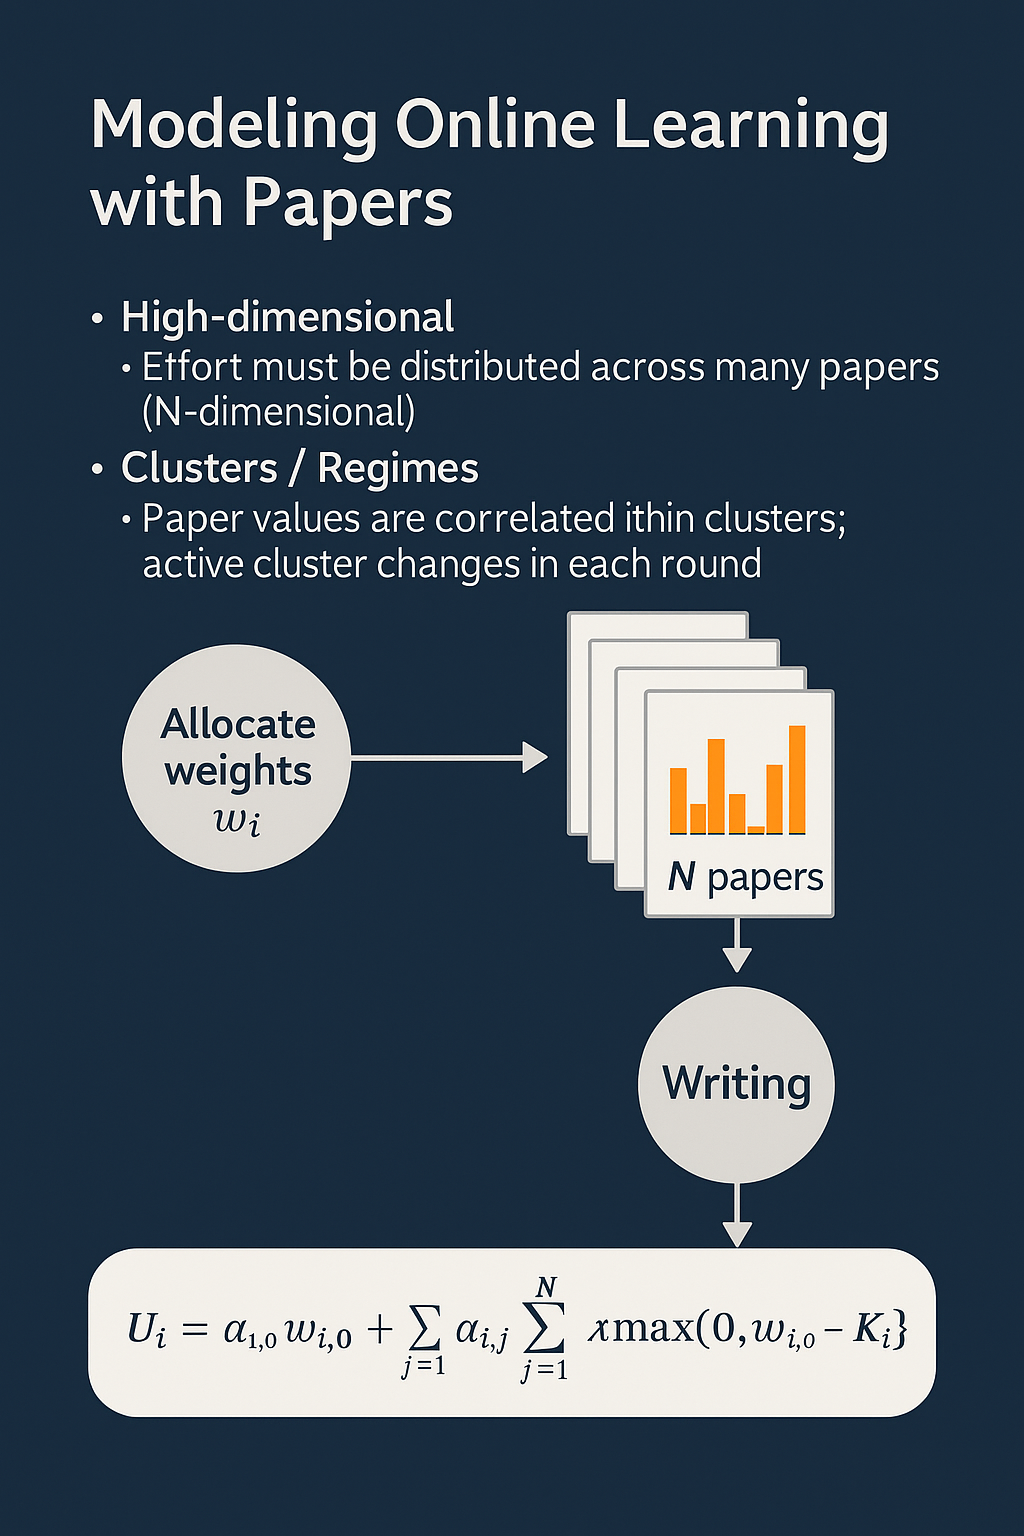
\includegraphics[width=0.35\linewidth]{332Project2/figures/Image_D.png}
    \caption{Image of D}
    \label{fig:placeholder}
\end{figure} 
\end{frame}

\begin{frame}{D - Game structure and Intuition}
Here's our Intuition;
\begin{itemize}
    \item 
\end{itemize}
\end{frame}

\begin{frame}{D - Parameters}
There is a intuitive meaning for each parameter.
\begin{itemize}
    \item N = 20 ; the number of papers reseacher reads
    \item h = 0.3 ; the frequency of regime change
    \item $\rho$ = 0.5 ; the correlation in a cluster
    \item $\lambda$ = 0.1 ; whichi is penalty for not reading enough before writing. 
\end{itemize}
\end{frame}

\begin{frame}{D - Results(Regrets)}

    
\end{frame}

\begin{frame}{D - Results(Payoffs)}

    
\end{frame}

\begin{frame}{D - Results(Regret bound)}

    
\end{frame}

\section{Reference and Usage of AI}
\begin{frame}{Reference and Usage of AI}
    Data we used is here.
    AI was used for coding, making images;\\
    final review and responsibility by the authors.
    
\end{frame}


\end{document}